\chapter{Bayesian deconvolution}
\label{chapt:bayesian-deconvolution}

Early stages of the SPHERE-2 analysis included an attempt to construct the process of estimating the parameters of an EAS photons in each PMT (the photon count and the arrival time distribution) directly from the recorded signal, but it was not successful for a number of reasons. Instead, the idea arose to carry out a full deconvolution, that is, to extract information about the photon flux at PMTs input at each moment of time. This deconvolution should take into account the stochastic properties of the PMT. Similar problems are also considered in other areas, for example, in the processing of \cite{Rhode1993} spectral measurements and \cite{Wipf2013} images. In such problems, Bayesian statistics is fruitfully used, based on the interpretation of probability as a measure of information about the random variable or confidence in its value \cite{Gelman2013}.

\section{Problem setup}

The input signal is modeled as a set of $\delta$-functions offsetted in time. Time bins ($12.5~\mathrm{nsec}$ in the SPHERE-2 detector) provide natural time scale, and we assume that within each time bin, $\delta$-functions are distributed uniformly. We limit ourselves with $N$ time bins. The deconvolution will yield estimation for $n_i$, photon counts per $[i-1, i]$ time bin, where $i = 1 \ldots N$.

We assume that the PMT is a linear system with stochastic impulse response function $\tilde{h}(t)$ in the sense that each of the $\delta$-functions that make up the input signal is convolved with an independent sample $h(t) \sim\tilde{h}(t)$. This corresponds to the idea of fluctuations in the PMT amplification happening independently for each electron cascade. We will assume that any sample from $\tilde{h}(t)$ is causal, i.e. $\forall t < 0 \; \; \forall h \sim \tilde{h} \; \; h(t) = 0$, and finite in time, i.e. $\exists \tilde{L}$ such that $\forall t > \tilde{L} \; \; \tilde{h}(t) = 0$. We will call this random function, which gives a new sample for each input $\delta$-function, the system's randomized impulse response (RIR).

We pose the problem of statistical deconvolution using Bayesian terminology

\begin{quote}
	Given the randomized impulse response of the system $\tilde{h}(t)$ and the output signal $s_j, \; j = 1, \ldots, N + L$, find the posterior probability density functions for the values $n_i$, $i = 1, \ldots, N$.
\end{quote}

Note that, unlike regular deconvolution, we are not trying to estimate the full original signal (sum of $\delta$-functions), but only its integrated in each time bin.

Mathematically, we write

\begin{equation}
	P(\vec{n} | \vec{s}) = \frac{P(\vec{s} | \vec{n}) \, P(\vec{n})}{P(\vec{s})}
\end{equation}

Using \textit{uninformative} prior $P(\vec{n}) = Const$ (it can't be normalized, but we will use only proportionality, not an absolute value), denoting likelihood function $\mathcal{L}(\vec{s}, \vec{n}) = P(\vec{s} | \vec{n})$, we get

\begin{equation}
	\label{eq:bayes-theorem-adapted}
	P(\vec{n} | \vec{s}) \propto \mathcal{L}(\vec{s}, \vec{n})
\end{equation}

\section{Likelihood function}
\label{sec:naive-monte-carlo-likelihood}

PMT output signal $\vec{s}$ is a sample from some multivariate random variable. Denoting this variable $\vec{S}$, we can write

\begin{equation}
	S_j = \sum_{l=0}^{L} C(n_{j-l}, l)
	\label{eq:S-definition-as-random-variable}
\end{equation}

Here $C(n, l)$ is a random variable describing the contribution of $n$ $\delta$-functions with the \textit{delay} of $l$ bins. It is easy to see from the chosen bin indexing scheme and the conditions of causality and boundedness in time of the RIH that $l \in \left[0, L\right]$, since the contribution from $\delta$-functions from earlier bins is equal to zero.

The distribution of $C(n, l)$ can be studied with Monte-Carlo. Sampling it goes as follows. If we sample RIR $h_k(t) \sim \tilde{h}(t)$ and in-bin time $t_{inbin} \sim U(0, 1)$, and get a sample from $C(1, l) = h_k(l + 1 - t_inbin)$. Sampling from $C(n, l)$ is trivial, since the system is linear and we can just add $n$ independent samples from $C(1, l)$.

To calculate likelihood function, one needs to find a probability to find a particular $\vec{s}$ sampling from $\vec{S}$. Naive Monte-Carlo likelihood estimation requires sampling a large number of $\vec{n}$ and computing histogram in $\vec{s}$ space. This method is computationally unfeasible, because of the curse of dimensionality: in practice we are interested in signals at least 50 time bins long.

\subsection{Multivariate normal distribution approximation}
\label{sec:likelihood-as-multivar-normal}

We approximate likelihood function with the multivariate normal distribution. There is no formal proof for the applicability for such approximation, but we estimate that it is fairly close for input intensities as low as 4-5 $\delta$-functions per bin, which is the characteristic background intensity in SPHERE-2 detector. For partial univariate $s_j$ distribution, the probability density function is within 1-2\% of its normal approximation.

The general form of multivariate normal distribution is

\begin{equation}
	\label{eq:multivariate-normal-density}
	p(\vec{s}) = \left( (2 \pi)^{N+L} \, \det \Sigma \right)^{-1/2} \exp \left( - \frac{1}{2} (\vec{s} - \vec{\mu})^T \Sigma^{-1} (\vec{s} - \vec{\mu}) \right)
\end{equation}

Here, mean vector $\vec{\mu}$ and covariance matrix $\Sigma$ depend on input $\vec{n}$ and RIR $\tilde{h}(t)$. Specifically, $\vec{\mu} \equiv \mathbb{E} \vec{S}$ can be obtained from \ref{eq:S-definition-as-random-variable} by computing mean of left and right terms and using the fact that $\mathbb{E} C(n, l) = n \; \mathbb{E} C(1, l)$. The matrix $\Sigma$ can be expressed in terms of $C(n, l)$ autocovariance, which can be further expressed in terms of $C(1, l)$ autocovariance. The latter depend only on RIR and not on $\vec{n}$, and can be pre-calculated for computational effectiveness.

\begin{equation}
	\Sigma_{ij} = \cov(S_i, S_j) = \sum_{l=0}^{L - (i-j)} \cov(C(n_{i-l}, l), C(n_{i-l}, l + (i-j)))
\end{equation}


\section{Output signal error}

Multivariate normal approximation does not account for the error of measuring the output signal. The largest contribution to this error is ADC discretization. We assume that ADC floors its input, i.e. for each recorded $s_j$, the real input value was somewhere between $s_j$ and $s_j + \delta$ and the distribution is uniform. Such error can be accounted for by integrating the $\mathcal{L}_{\mathrm{exact}}(\vec{s}, \vec{n})$ defined by \ref{eq:multivariate-normal-density} over the $N$-dimensional cube with side $\delta$ and <<lower>> corner at $\vec{s}$:

\begin{equation}
	\label{eq:likelihood-with-error-uniform-error}
	\mathcal{L}(\vec{s}, \vec{n}) = \int_{s_1}^{s_1 + \delta} \int_{s_2}^{s_2 + \delta} \ldots \, \int_{s_{N}}^{s_N + \delta} \mathcal{L}_{\mathrm{exact}}(\vec{s}, \vec{n}) \, d\vec{s}
\end{equation}

To perform this integration numerically, we use the ready-made adaptive integration algorithm described in \cite{Genz1992}, implemented in the \texttt{scipy.stats} \cite{2020SciPy-NMeth} \texttt{Python} package.


\section{Posterior distribution sampling}
\label{sec:mcmc-sampling}

Having obtained the likelihood function $\mathcal{L}$, we can estimate $\vec{n}$ given the recorded output signal $\vec{s}$ and RIR $\tilde{h}(t)$. We want not only to find the optimal value of $\vec{n}$, but also characterize our confidence in it.

Instead of maximum likelihood method, where we would maximize the value of $\mathcal{L}(\vec{n}, \vec{s})$ with respect to $\vec{n}$, we use Marko Chain Monte Carlo sampling to draw a large sample from $P(\vec{n} | \vec{s}) \propto \mathcal{L}(\vec{n}, \vec{s})$. Using this sample of possible $\vec{n}$ values, we will then get the bets-fitting value for system's input, and its error.

The idea of the Markov Chain Monte Carlo (MCMC) family of methods \cite{Sharma2017} is to launch a Markov process (random walk) in the parameter space $\vec{n}$ with transition probability chosen in such a way that the <<trace>> of the walk will yield a sample from the target probability density functions. A common characteristic of this family is that they require only knowing only a ratio of probability density functions at different points in the parameter space, which is why in the expression (\ref{eq:bayes-theorem-adapted}) and in all subsequent calculations we were able to drop the marginal probability and the normalization of the prior distribution.

The particular method used in this work is affine-invariant MCMC \cite{Goodman2010}, implemented in \verb|Python| package \verb|emcee| \cite{ForemanMackey2016}.

\section{Deconvolution results}

A detailed description of the PMT connection and power supply circuits, the amplification circuit, as well as the characteristics of the used ADC converters can be found in \cite{SphereDetector2020}. For purposes of this work, we define detector's randomized impulse response as 

\begin{equation}
	\label{eq:experimental-rir}
	\tilde{h}(t) = C \, \tilde{C}_{PMT} \, h_I(t)
\end{equation}

\begin{figure}
	\centering
	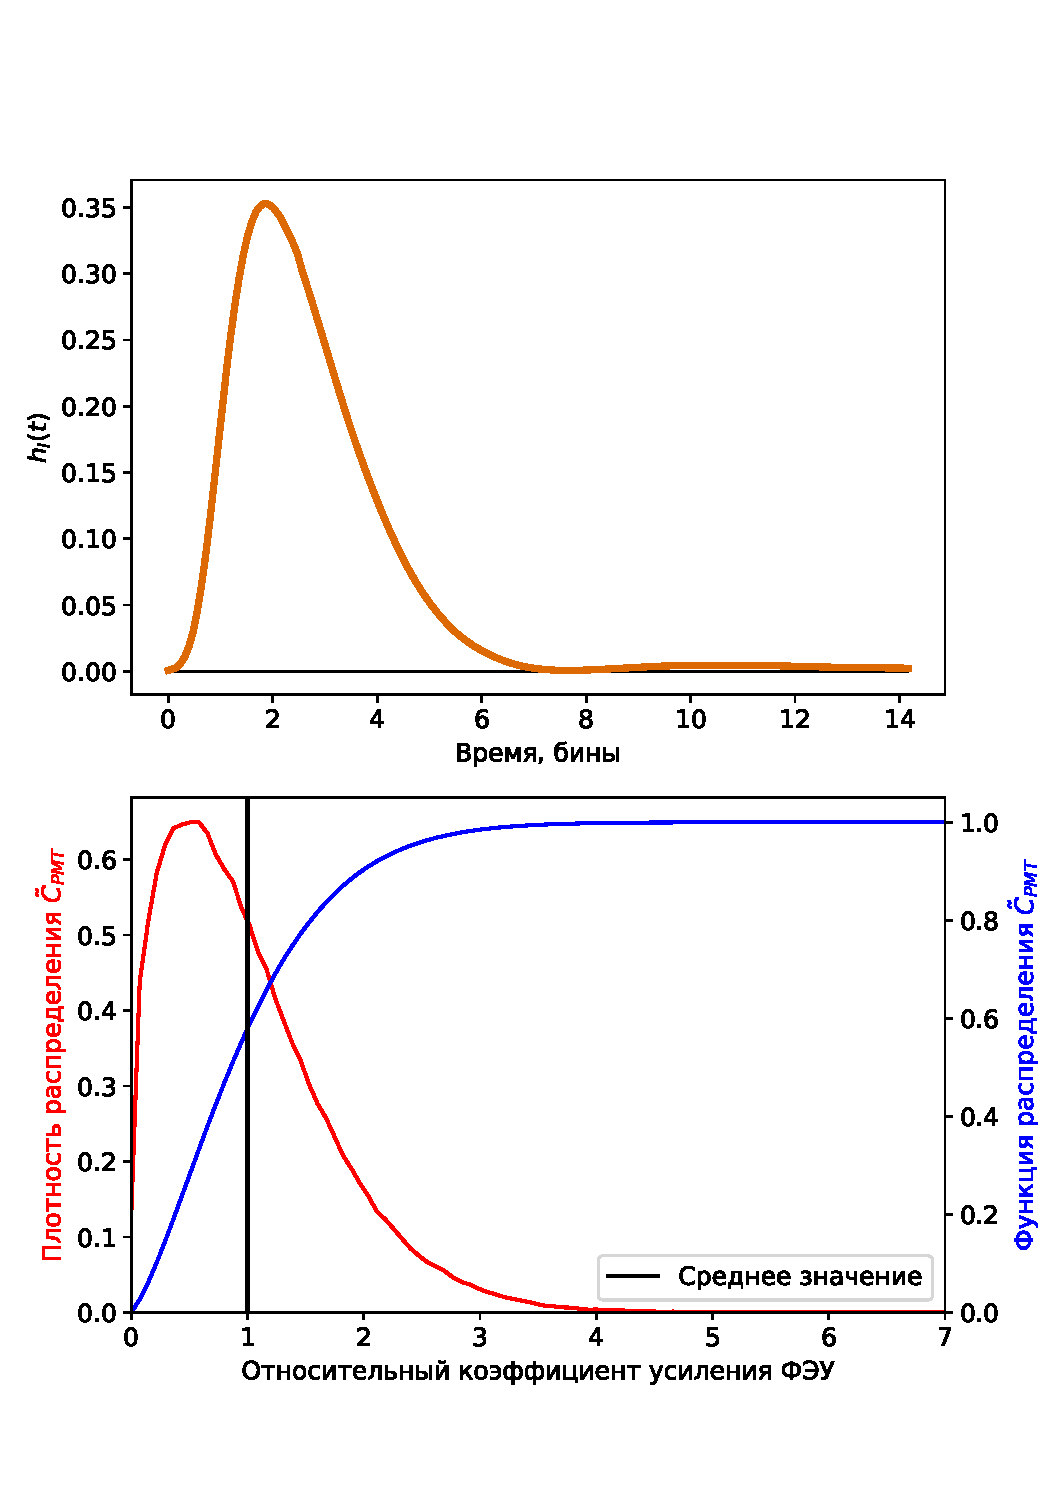
\includegraphics[width=0.85\columnwidth]{experimental-ir-params}
	\caption{SPHERE-2 PMT's randomized impulse response. $h_I(t)$ (top panel) is the signal's shape in time domain, $\tilde{C}_{PMT}$ (bottom panel: PDF and CDF) --- dimensionless random PMT amplification coeffient.}
	\label{pic:experimental-rir-params}
\end{figure}

Where

\begin{enumerate}
	\item $h_I(t)$ --- shape of the impulse response, defined by time characteristics of the PMT and signal amplification circuit. Measured in the laboratory and plotted on the top panel of Fig. \ref{pic:experimental-rir-params}. Normalized to have integral 1.
	\item $\tilde{C}_{PMT}$ --- dimensionless random PMT amplification coefficient, normalized to have a mean value of 1. It's PDF and CDF are plotted on the bottom panel of Fig. \ref{pic:experimental-rir-params}.
	\item $C$ --- scale coefficient. It is measured during detector calibration and applied to signals earlier in data processing pipeline.
\end{enumerate}

We illustrate deconvolution procedure on toy input data: Poisson background with mean $\lambda=20$ photons per time bin and a <<signal>> photon packet: 3 bins with additional Poisson signal with $\lambda_{\mathrm{signal}}=40$. Fig. \ref{pic:bayesian-deconvolution-with-experimantal-rir-and-rounding} illustrates the system's input and output on the top panel and the deconvolution results on the bottom panel.


\begin{figure}
	\centering
	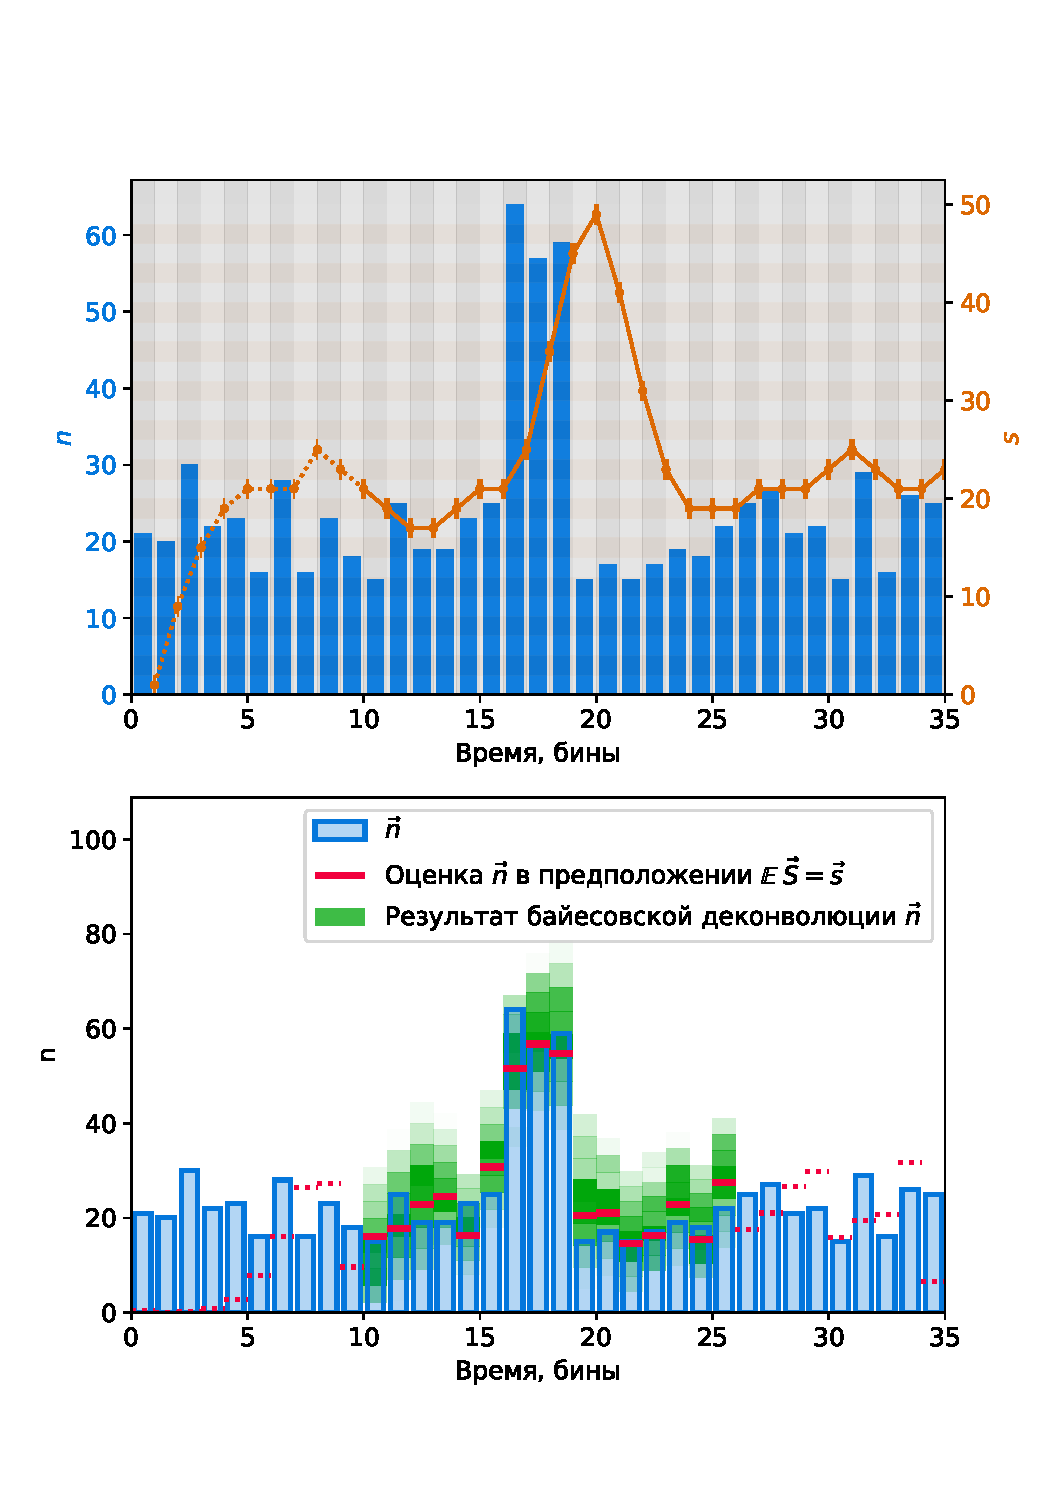
\includegraphics[width=0.85\columnwidth]{final-problem-and-solution}
	\caption{Bayesian deconvolution performed on synthetic toy input data. \textbf{Top panel:} toy input data $\vec{n}$ (blue) and corresponding system's output (convolution with randomized impulse response from fig. \ref{pic:experimental-rir-params}) $\vec{s}$, orange (X axis: <<Time, bins>>). \textbf{Bottom pannel}: same input data $\vec{n}$ (blue); rough $\vec{n}$ estimation from mean values, MCMC sampling starting point (red); deconvolution result, marginal posterior distributions in each time bin (green).}
	\label{pic:bayesian-deconvolution-with-experimantal-rir-and-rounding}
\end{figure}

